\documentclass[landscape]{article}
\usepackage[pdftex]{graphicx}
\usepackage[utf8]{inputenc}
\usepackage{enumerate}
\usepackage{icomma}
\usepackage{amssymb}
\usepackage{tikz}
\usepackage{href-ul}
\hypersetup{
	colorlinks=true,
	linkcolor=blue,
	urlcolor=blue}
\usepackage{geometry}
\geometry{a4paper, top=15mm, left=15mm, right=15mm, bottom=15mm,
	headsep=10mm, footskip=12mm}
\twocolumn

\begin{document}
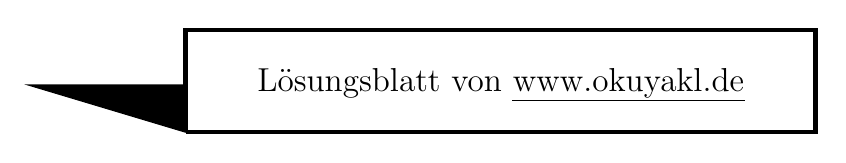
\begin{tikzpicture}(10,3)
	\draw[ultra thick](2,0) --(10,0) -- (10,1.3) --(2,1.3) -- (2,0);
	\draw[fill=black](2,0)-- (0,.6) -- (2,.6) -- (2,0);
	\node at (6,.6) {\large Lösungsblatt von \href{https://www.okuyakl.de}{www.okuyakl.de}};
\end{tikzpicture}
\vspace{0.5 cm}

\noindent{\bf Aufgabe 1. a)}\\
$$
\renewcommand{\arraystretch}{2}
\begin{array}{rcll}
\sin(\alpha + 60^\circ) &=& {3 \over 6} & | \sin^{-1} \\
\alpha_1 + 60^\circ &=& 30^\circ \quad (*) &  | - 60^\circ \\
\alpha_1 &=& -30^\circ & | +360^\circ \\
\alpha_1 &=& 330^\circ \\
(*)\quad 180^\circ -(\alpha_2+ 60^\circ) &=& 30^\circ \\
120^{\circ}-\alpha_2 &=& 30^\circ \\
\alpha_2 &=& 90^\circ 
\end{array}\\
\mathbb{L}=\{90^\circ ;330^\circ \}
$$
\noindent{\bf Aufgabe 1. b)}\\
$$
\renewcommand{\arraystretch}{2}
\begin{array}{rcll}
\cos(\alpha +45^\circ)&=&{2 \over 2} & |\cos^{-1}\\
\alpha_1 +45^\circ &=& 0^\circ &\quad (*)\\
\alpha_1 &=& -45^\circ &| +360^\circ \\
\alpha_1 &=& 315^\circ \\
(*) \quad 360^\circ - (\alpha_2+45^\circ) &=& 0^\circ \\
315^\circ - \alpha_2 &=&  0^\circ \\
\alpha_2 &=& 315^\circ &=\alpha_1 \\
\end{array}\\
\mathbb{L}=\{ 315^\circ \}
$$

\newpage
\noindent{\bf Aufgabe 1. c)}\\
$$
\renewcommand{\arraystretch}{2}
\begin{array}{rcll}
\sin^2\alpha &=&0,75& |\pm \sqrt{\quad} \\
\sin\alpha &=& \sqrt{0,75}&|\sin^{-1} \\
\alpha_1 &=& 60^\circ \\
\alpha_2 &=& 180^\circ - 60^\circ&= 120^\circ\\
\alpha_3 &=& -60^\circ &| +360^\circ\\
\alpha_3 &=& 300^\circ\\
\alpha_4 &=& 180^\circ-(-60^\circ)&=240^\circ\\
\end{array}\\
\mathbb{L}=\{60^\circ;120^\circ; 240^\circ; 300^\circ \}
$$

\noindent{\bf Aufgabe 1. d)}\\
$$ \sin\alpha + \cos\alpha = 2$$
Es gibt keinen Winkel, für den dies gilt, weil Sinus und Kosinus an verschiedenen Stellen 1 sind.
$$\mathbb{L}=\{ \}$$

\noindent{\bf Aufgabe 1. e)}\\
$$
\renewcommand{\arraystretch}{2}
\begin{array}{rcll}
1-\cos^2\alpha &=& 0\\
\cos^2\alpha &=& 1 & \pm \sqrt{\quad}\\
\cos\alpha_1 &=& 1 \\ 
\alpha_1 &=& 0^\circ\\
\alpha_2 &=& 360^\circ\\
\cos\alpha_3 &=& -1 \\
\alpha_3 &=& 180^\circ\\
\end{array}\\
\mathbb{L}=\{0^\circ; 180^\circ ; 360^\circ \}
$$

\newpage
\noindent{\bf Aufgabe 1. f)}\\
Wir wenden die dritte Binomische Formel an:
$$
\renewcommand{\arraystretch}{2}
\begin{array}{rcll}
\sin^2\alpha -0,36 &=& 0,28 \\
\sin^2\alpha &=& 0,64 &|\sqrt{\quad}\\
\sin\alpha &=& \pm 0,8 \\
\alpha_1 &=& 53,13^\circ \\
\alpha_2 &=& -53,13^\circ &= 306,87^\circ \\
\alpha_3 &=& 180^\circ-53.13^\circ &= 126,87^\circ\\
\alpha_4 &=& 180^\circ-(-53.13^\circ) &= 233,13^\circ\\
\end{array}\\
\mathbb{L}=\{53,13^\circ; 126,87^\circ; 233,13^\circ \}
$$

\noindent{\bf Aufgabe 1. g)}\\
Ab dieser Aufgabe müssen wir die Additionstheoreme heranziehen; aus einem folgt:
$\sin(2\alpha)=2\cdot\sin\alpha\cdot\cos\alpha$
$$
\renewcommand{\arraystretch}{2}
\begin{array}{rcll}
\sin(2\alpha)&=&0,5\\
2\alpha_1 &=& 30^\circ \\
\alpha_1 &=& 15^\circ \\
180^\circ-2\alpha_2 &=& 30^\circ\\
2\alpha_2 &=& 150^\circ \\
\alpha_2 &=& 75^\circ 
\end{array}\\
\mathbb{L}=\{15^\circ; 75^\circ  \}
$$

\newpage
\noindent{\bf Aufgabe 1. h)}\\
Aus den Additionstheoremen folgt auch: $\cos(2\alpha)=\cos^2\alpha-\sin^2\alpha$
$$
\renewcommand{\arraystretch}{2}
\begin{array}{rcll}
\cos\alpha &=& \sin\alpha& |:\cos{\alpha}\\
1&=&{ \sin\alpha \over \cos\alpha}\\
1&=&\tan\alpha& |\tan^{-1}\\
\alpha_1 &=& 45^\circ\\
\alpha_2 &=&180^\circ+45^\circ&= 225^\circ
\end{array}\\
\mathbb{L}=\{45^\circ; 225^\circ  \}
$$

\noindent{\bf Aufgabe 1. i)}\\
Wir haben eine quadratische Gleichung und substituieren mit $u=\sin\alpha$:
$$4u^2 + 4u +1 =0$$
Die Mitternachtsformel liefert:
$$u_{1/2}=0,5$$
Wir können rücksubstituieren:
$$\sin\alpha={0,5} \Rightarrow \alpha_1 =30^\circ; \alpha_2=150^\circ$$
$$\mathbb{L}=\{30^\circ;150^\circ \}$$ 

\noindent{\bf Aufgabe 1. j)}\\
Wir teilen durch 2:
$$\renewcommand{\arraystretch}{2}
\begin{array}{rcll}
\sin{\alpha\over 2} &=& 0\\
{\alpha_1\over 2} &=& 0 \\
\alpha_1 &=& 0\\
{\alpha_2 \over 2} &=&180^\circ \\
\alpha_2 &=& 360^\circ &= 0^\circ\\
{\alpha_3 \over 2} &=&360^\circ \\
\alpha_3 &=& 720^\circ &=0^\circ \\
\end{array}\\
\mathbb{L}=\{0^\circ; 360^\circ \}
$$
 
\newpage
\noindent{\bf Aufgabe 1. k)}\\
Gleiche Zähler links und rechts, also können wie direkt die Nenner gleichsetzen:
$$
\renewcommand{\arraystretch}{2}
\begin{array}{rcll}
4 \sin\gamma&=& 3\\
\sin(\gamma) &=& {3\over 4}\\
\gamma_1 &=&  48,59^\circ \\
\gamma_2) &=& 180^\circ - 48,59^\circ \\
\gamma_2 &=& 131,41^\circ
\end{array}\\
\mathbb{L}=\{48,59^\circ; 131,41^\circ \}
$$

\noindent{\bf Aufgabe 1. l)}\\
Wir stellen um und wenden ein Additionstheorem an:
$$
\renewcommand{\arraystretch}{2}
\begin{array}{rcll}
\sin\epsilon &=& 4 \sqrt{3}\cdot (\sin\epsilon \cos(30^\circ)+\sin(30^\circ)\cos\epsilon)\\
\sin\epsilon &=& 4 \sqrt{3}\cdot (\sin\epsilon {1\over 2}\sqrt{3} + {1\over 2}\cos\epsilon)\\
\sin\epsilon &=& 2\cdot 3 \cdot \sin\epsilon +2 \sqrt{3} \cos\epsilon\\
-5 \sin\epsilon &=& 2 \sqrt{3} \cos\epsilon &|:\cos\epsilon \quad|:(-5)\\
\tan\epsilon &=& -{2\over 5}\sqrt{3}\\
\epsilon_1 &=& -34,71^\circ\\
\epsilon_1 &=& 325,29^\circ\\
\epsilon_2 &=& 180^\circ-34,71^\circ = 145,29^\circ\\
\end{array}\\
\mathbb{L}=\{145,29^\circ; 325,29^\circ  \}
$$

\begin{center}
	\includegraphics[width=7 cm]{../../viecher/endcomic.pdf}
	
	Hier geht es zurück zum \href{https://www.okuyakl.de/math/m10gonL082/aa082.pdf}{Aufgabenblatt}
\end{center}


%Ende
\end{document}